\documentclass[tikz,border=5mm]{standalone}
\usepackage{fontspec}
\setmainfont{Hiragino Sans}
\usepackage{xcolor}

\begin{document}
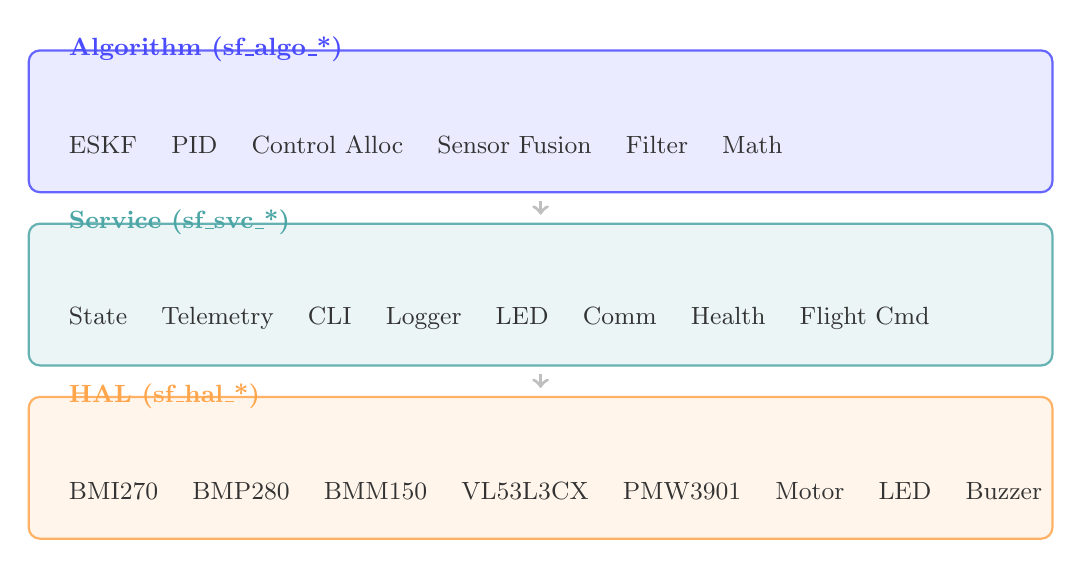
\begin{tikzpicture}[
  layer/.style={
    draw=#1!60, fill=#1!8, rounded corners=4pt,
    minimum width=130mm, minimum height=18mm,
    font=\large, align=center, line width=0.8pt
  },
  label/.style={
    font=\small\bfseries, text=#1!70
  },
  item/.style={
    font=\small, text=black!80
  }
]

% Algorithm layer
\node[layer=blue] (algo) at (0, 0) {};
\node[label=blue, anchor=west] at ([xshift=4mm]algo.north west) {Algorithm (sf\_algo\_*)};
\node[item, anchor=west] at ([xshift=4mm, yshift=-3mm]algo.west) {ESKF \quad PID \quad Control Alloc \quad Sensor Fusion \quad Filter \quad Math};

% Service layer
\node[layer=teal] (svc) at (0, -2.2) {};
\node[label=teal, anchor=west] at ([xshift=4mm]svc.north west) {Service (sf\_svc\_*)};
\node[item, anchor=west] at ([xshift=4mm, yshift=-3mm]svc.west) {State \quad Telemetry \quad CLI \quad Logger \quad LED \quad Comm \quad Health \quad Flight Cmd};

% HAL layer
\node[layer=orange] (hal) at (0, -4.4) {};
\node[label=orange, anchor=west] at ([xshift=4mm]hal.north west) {HAL (sf\_hal\_*)};
\node[item, anchor=west] at ([xshift=4mm, yshift=-3mm]hal.west) {BMI270 \quad BMP280 \quad BMM150 \quad VL53L3CX \quad PMW3901 \quad Motor \quad LED \quad Buzzer};

% (arrows drawn below with better visibility)

% Arrows - make more visible
\draw[->, very thick, gray!50] ([yshift=-1mm]algo.south) -- ([yshift=1mm]svc.north);
\draw[->, very thick, gray!50] ([yshift=-1mm]svc.south) -- ([yshift=1mm]hal.north);

\end{tikzpicture}
\end{document}
